% STATUS: ACTIVE -- 2026-10-23 (user): three-axis estimator written entirely in the measurement coordinate (x, y, z). States: tracking
%   error delay chain and the six entries of the motion gain matrix A-bar; the wall angles are NOT states, they are computed every step
%   from the estimated A-bar (closed form from the trace and the sum of squares; 10-23 the incremental small-angle form locked onto
%   wrong eigenvectors in the first test, 23 / 36 cells, and moved to the appendix). Part A = one-step algorithm in the order of the notes "Estimation and
%   Control_R" (Word); Part B = key derivation steps. Kept short on purpose (user 10-23): no Q, R, P[0], init, values; no a-bar' (gain
%   change with height), delay chain d = 2 kept. Previous version with the angles as states: 1015_estimator_3d_wsonly.tex.
%   New symbols (user 10-23): a-bar (bold) = the six entries of A-bar; left superscript v on A-hat = A-hat seen in the previous ruler
%   (appendix only); t, s = trace and sum of squares of A-hat (A5).
% Compile: xelatex 1023_estimator_3d_xyz.tex (from reference/eq17_analysis/derivation/). Preamble from 1015_estimator_3d_wsonly.tex.
\documentclass[11pt,a4paper]{ctexart}
\usepackage[fleqn]{amsmath}
\usepackage{amssymb,bm,graphicx,booktabs}
\setlength{\mathindent}{0pt}
\usepackage{geometry}
\geometry{margin=1.8cm}
\setlength{\parindent}{0pt}
\setlength{\parskip}{0.2em}
\usepackage{xcolor}
\graphicspath{{figures/}}
\newcommand{\setline}[1]{\noindent{\small\textcolor[gray]{0.35}{#1}}\par\smallskip}
\newcommand{\hd}[1]{\par\bigskip\noindent\underline{\textbf{#1}}}
\newcommand{\lc}{\lambda_c}
\newcommand{\bp}{\bar{\mathbf p}}
\newcommand{\dpb}{\delta\bar{\mathbf p}}
\newcommand{\dph}{\delta\hat{\bar{\mathbf p}}}
\newcommand{\Ab}{\bar{\mathbf A}}
\newcommand{\Ah}{\hat{\bar{\mathbf A}}}
\newcommand{\vAh}{{}^{v}\!\hat{\bar{\mathbf A}}}
\newcommand{\av}{\bar{\mathbf a}}
\newcommand{\avh}{\hat{\bar{\mathbf a}}}
\newcommand{\uu}{\mathbf u}
\newcommand{\vv}{\mathbf v}
\newcommand{\ww}{\mathbf w}
\newcommand{\aT}{\bar a_T}
\newcommand{\aN}{\bar a_N}
\newcommand{\haT}{\hat{\bar a}_T}
\newcommand{\haN}{\hat{\bar a}_N}
\newcommand{\Fd}{\bar{\mathbf F}_{dp}}
\newcommand{\epp}{\boldsymbol\varepsilon_p}
\newcommand{\I}{\mathbf I}
\newcommand{\Sn}{\boldsymbol\Sigma_n}
\newcommand{\CK}{C_T\,\kappa_T}
\newcommand{\E}{\mathrm{E}}
\newcommand{\V}{\mathbf V}
\newcommand{\Vh}{\hat{\mathbf V}}
\newcommand{\Lb}{\bar{\boldsymbol\Lambda}}
\pagestyle{plain}

\begin{document}

\begin{center}\textbf{\large Three-axis estimator in the measurement coordinate}\\[2pt]
\small 2026-10-23 \quad states in $(x, y, z)$: tracking error and the motion gain matrix $\Ab$; wall angles computed from $\Ah$\end{center}

\setline{Part A: one step of the algorithm (order of the notes). Part B: the key derivation steps. Q, R, $\mathbf P[0]$ and initial values are not written here.}

%======================================================================
\part*{Part A \quad One step of the algorithm}

\hd{A1 \quad Input and measurement}
\begin{align*}
&\bp_d[k],\ \ \bp_d[k+1] \\
&\bp_m[k] \\
\dpb_m[k] &= \bp_d[k-d] - \bp_m[k]
\end{align*}

\hd{A2 \quad Control law}
\begin{align*}
\hat{\bp}[k] &= \bp_m[k] + \sum_{i=1}^{d} \Ah[k-i]\,\bar{\mathbf f}_d[k-i] \\
\bar{\mathbf f}_d[k] &= \Ah^{-1}[k]\,\Big\{\bp_d[k+1] - \hat{\bp}[k] - \lc\,\big(\bp_d[k] - \hat{\bp}[k]\big)\Big\}
\end{align*}

\hd{A3 \quad Deterministic and random components, measured motion gain matrix}
\begin{align*}
\overline{\dpb_m}[k+1] &= a_{\mathrm{pd}}\,\dpb_m[k] + (1 - a_{\mathrm{pd}})\,\overline{\dpb_m}[k] \\
\dpb_r[k] &= \dpb_m[k] - \overline{\dpb_m}[k] \\
\Ab_m[k] &= \frac{\dpb_r[k]\,\dpb_r^{T}[k] - C_n\,\Sn}{\CK} \\
\av_m[k] &= \big[\,[\Ab_m]_{xx}\ \ [\Ab_m]_{yy}\ \ [\Ab_m]_{zz}\ \ [\Ab_m]_{xy}\ \ [\Ab_m]_{xz}\ \ [\Ab_m]_{yz}\,\big]^{T}
\end{align*}

\hd{A4 \quad Estimation error and state update}
\begin{align*}
\mathbf y[k] &= \begin{bmatrix} \dpb_m[k] \\ \av_m[k] \end{bmatrix}, \qquad
\hat{\mathbf y}[k] = \begin{bmatrix} \dph_1[k] \\ \avh[k] \end{bmatrix}, \qquad
\mathbf e_y[k] = \mathbf y[k] - \hat{\mathbf y}[k] \\
\mathbf L[k] &= \mathbf P^f[k]\,\mathbf H^{T}\big(\mathbf H\,\mathbf P^f[k]\,\mathbf H^{T} + \mathbf R[k]\big)^{-1} \\
\dph_1[k+1] &= \dph_2[k] + \mathbf L_1[k]\,\mathbf e_y[k] \\
\dph_2[k+1] &= \dph_3[k] + \mathbf L_2[k]\,\mathbf e_y[k] \\
\dph_3[k+1] &= \lc\,\dph_3[k] + \mathbf L_3[k]\,\mathbf e_y[k] \\
\avh[k+1] &= \avh[k] + \mathbf L_4[k]\,\mathbf e_y[k]
\end{align*}
\setline{$\mathbf L_1, \mathbf L_2, \mathbf L_3$: $3\times 9$; $\mathbf L_4$: $6\times 9$. $\Ah[k+1]$ is the symmetric matrix built from $\avh[k+1]$.}

\hd{A5 \quad Wall angles from the estimated motion gain matrix}
\begin{align*}
t[k+1] &= \hat{\bar a}_{xx} + \hat{\bar a}_{yy} + \hat{\bar a}_{zz} \\
s[k+1] &= \hat{\bar a}_{xx}^{2} + \hat{\bar a}_{yy}^{2} + \hat{\bar a}_{zz}^{2} + 2\,\hat{\bar a}_{xy}^{2} + 2\,\hat{\bar a}_{xz}^{2} + 2\,\hat{\bar a}_{yz}^{2} \\
\haT[k+1] &= \frac{2\,t[k+1] + \sqrt{6\,s[k+1] - 2\,t^{2}[k+1]}}{6} \\
\haN[k+1] &= t[k+1] - 2\,\haT[k+1] \\
\hat\ww[k+1] &= \pm\,\frac{\mathbf c}{\|\mathbf c\|}, \qquad
\mathbf c = \begin{bmatrix} \hat{\bar a}_{xz} \\ \hat{\bar a}_{yz} \\ \hat{\bar a}_{zz} - \haT[k+1] \end{bmatrix}, \qquad \hat w_z > 0 \\
\hat\theta_x[k+1] &= -\arcsin \hat w_y \\
\hat\theta_y[k+1] &= \mathrm{atan2}\big(\hat w_x,\ \hat w_z\big) \\
\Vh[k+1] &= \mathbf R_y\big(\hat\theta_y[k+1]\big)\,\mathbf R_x\big(\hat\theta_x[k+1]\big) = [\,\hat\uu\ \ \hat\vv\ \ \hat\ww\,]
\end{align*}
\setline{$\Vh$ is used only here and for commands along $\hat\ww$, $\hat\uu$; the estimator (A1--A4, A6) does not use it.}

\hd{A6 \quad Error covariance}
\begin{align*}
\mathbf P[k] &= \big(\I - \mathbf L[k]\,\mathbf H\big)\,\mathbf P^f[k] \\
\mathbf P^f[k+1] &= \mathbf F_e[k]\,\mathbf P[k]\,\mathbf F_e^{T}[k] + \mathbf Q[k]
\end{align*}

%======================================================================
\clearpage
\part*{Part B \quad Key derivation steps}

\section{Motion gain matrix of a tilted wall}
\begin{align*}
\V &= \mathbf R_y(\theta_y)\,\mathbf R_x(\theta_x) = [\,\uu\ \ \vv\ \ \ww\,] \\
\ww &= \begin{bmatrix} \sin\theta_y\cos\theta_x \\ -\sin\theta_x \\ \cos\theta_y\cos\theta_x \end{bmatrix} \\
\Lb &= \mathrm{diag}(\aT,\ \aT,\ \aN) \\
\Ab &= \V\,\Lb\,\V^{T} = \aT\,\I + (\aN - \aT)\,\ww\,\ww^{T} \\
\Lb &= \V^{T}\,\Ab\,\V
\end{align*}

%======================================================================
\section{The wall angles are the off-diagonal entries of $\Ab$}
\setline{Small angles: drop every product of two angles.}
\begin{align*}
\ww &\approx \begin{bmatrix} \theta_y \\ -\theta_x \\ 1 \end{bmatrix} \\
\ww\,\ww^{T} &\approx \begin{bmatrix} 0 & 0 & \theta_y \\ 0 & 0 & -\theta_x \\ \theta_y & -\theta_x & 1 \end{bmatrix} \\
\Ab &\approx \begin{bmatrix}
\aT & 0 & -(\aT - \aN)\,\theta_y \\
0 & \aT & (\aT - \aN)\,\theta_x \\
-(\aT - \aN)\,\theta_y & (\aT - \aN)\,\theta_x & \aN
\end{bmatrix} \\
\big[\Ab\big]_{xz} &\approx -(\aT - \aN)\,\theta_y \\
\big[\Ab\big]_{yz} &\approx (\aT - \aN)\,\theta_x \\
\big[\Ab\big]_{xy} &\approx 0
\end{align*}

%======================================================================
\clearpage
\section{Process: control law and tracking error}
\begin{align*}
\bp[k+1] &= \bp[k] + \Ab\,\big(\bar{\mathbf f}_d[k] + \bar{\mathbf f}_T[k]\big) \\
\dpb[k] &= \bp_d[k] - \bp[k] \\
\bp_m[k] &= \bp[k-d] + \mathbf n_p[k] \\
\dpb_m[k] &= \bp_d[k-d] - \bp_m[k] \\
\hat{\bp}[k] &= \bp_m[k] + \sum_{i=1}^{d} \Ah[k-i]\,\bar{\mathbf f}_d[k-i] \\
\bar{\mathbf f}_d[k] &= \Ah^{-1}[k]\,\Big\{\bp_d[k+1] - \hat{\bp}[k] - \lc\,\big(\bp_d[k] - \hat{\bp}[k]\big)\Big\} \\
\dpb[k+1] &= \lc\,\dpb[k] - \big(\Ab - \Ah[k]\big)\,\Fd[k] - \epp[k] \\
\Fd[k] &= \bar{\mathbf f}_d[k] + (1-\lc)\sum_{i=1}^{d} \bar{\mathbf f}_d[k-i]
\end{align*}

\hd{True state of the process}
\begin{align*}
\dpb_1[k+1] &= \dpb_2[k] \\
\dpb_2[k+1] &= \dpb_3[k] \\
\dpb_3[k+1] &= \lc\,\dpb_3[k] - \big(\Ab - \Ah[k]\big)\,\Fd[k] - \epp[k] \\
\av[k+1] &= \av[k] + \mathbf w_a[k]
\end{align*}

%======================================================================
\section{State vector and estimator}
\begin{align*}
\av &= \big[\,\bar a_{xx}\ \ \bar a_{yy}\ \ \bar a_{zz}\ \ \bar a_{xy}\ \ \bar a_{xz}\ \ \bar a_{yz}\,\big]^{T} \\
\mathbf x[k] &= \big[\,\dpb_1^{T}[k]\ \ \dpb_2^{T}[k]\ \ \dpb_3^{T}[k]\ \ \av^{T}[k]\,\big]^{T} \qquad (15 \times 1,\ d = 2)
\end{align*}
\begin{align*}
\dph_1[k+1] &= \dph_2[k] + \mathbf L_1[k]\,\mathbf e_y[k] \\
\dph_2[k+1] &= \dph_3[k] + \mathbf L_2[k]\,\mathbf e_y[k] \\
\dph_3[k+1] &= \lc\,\dph_3[k] + \mathbf L_3[k]\,\mathbf e_y[k] \\
\avh[k+1] &= \avh[k] + \mathbf L_4[k]\,\mathbf e_y[k]
\end{align*}

%======================================================================
\clearpage
\section{Dynamics of estimation errors}
\setline{$\mathbf e_{(\cdot)} = (\cdot) - (\hat\cdot)$; $\mathbf e_a = \av - \avh = [\,e_{xx}\ e_{yy}\ e_{zz}\ e_{xy}\ e_{xz}\ e_{yz}\,]^{T}$; $F_x, F_y, F_z$ = components of $\Fd[k]$}
\begin{align*}
\Ab - \Ah &= \begin{bmatrix} e_{xx} & e_{xy} & e_{xz} \\ e_{xy} & e_{yy} & e_{yz} \\ e_{xz} & e_{yz} & e_{zz} \end{bmatrix} \\
\big(\Ab - \Ah\big)\,\Fd &= \begin{bmatrix}
e_{xx}\,F_x + e_{xy}\,F_y + e_{xz}\,F_z \\
e_{xy}\,F_x + e_{yy}\,F_y + e_{yz}\,F_z \\
e_{xz}\,F_x + e_{yz}\,F_y + e_{zz}\,F_z
\end{bmatrix}
= \begin{bmatrix}
F_x & 0 & 0 & F_y & F_z & 0 \\
0 & F_y & 0 & F_x & 0 & F_z \\
0 & 0 & F_z & 0 & F_x & F_y
\end{bmatrix} \mathbf e_a
\end{align*}
\begin{align*}
\mathbf e_1[k+1] &= \mathbf e_2[k] \\
\mathbf e_2[k+1] &= \mathbf e_3[k] \\
\mathbf e_3[k+1] &= \lc\,\mathbf e_3[k] -
\begin{bmatrix}
F_x & 0 & 0 & F_y & F_z & 0 \\
0 & F_y & 0 & F_x & 0 & F_z \\
0 & 0 & F_z & 0 & F_x & F_y
\end{bmatrix} \mathbf e_a[k] - \epp[k] \\
\mathbf e_a[k+1] &= \mathbf e_a[k] + \mathbf w_a[k]
\end{align*}
\begin{align*}
\mathbf e[k+1] &= \mathbf F_e[k]\,\mathbf e[k] - \mathbf L[k]\,\mathbf H\,\mathbf e[k] + \mathbf q[k] \\
\mathbf F_e[k] &=
\begin{bmatrix}
\mathbf 0 & \I_3 & \mathbf 0 & \mathbf 0 \\
\mathbf 0 & \mathbf 0 & \I_3 & \mathbf 0 \\
\mathbf 0 & \mathbf 0 & \lc\,\I_3 &
-\begin{bmatrix}
F_x & 0 & 0 & F_y & F_z & 0 \\
0 & F_y & 0 & F_x & 0 & F_z \\
0 & 0 & F_z & 0 & F_x & F_y
\end{bmatrix} \\
\mathbf 0 & \mathbf 0 & \mathbf 0 & \I_6
\end{bmatrix} \\
\mathbf q[k] &= \big[\,\mathbf 0^{T}\ \ \mathbf 0^{T}\ \ -\epp^{T}[k]\ \ \mathbf w_a^{T}[k]\,\big]^{T}
\end{align*}

%======================================================================
\clearpage
\section{Process outputs and output matrix}
\begin{align*}
\E\big[\dpb_r\,\dpb_r^{T}\big] &= \CK\,\Ab + C_n\,\Sn \\
\E\big[\Ab_m\big] &= \Ab \\
\E\big[\av_m\big] &= \av
\end{align*}
\[
\mathbf y[k] = \begin{bmatrix} \dpb_m[k] \\ \av_m[k] \end{bmatrix},
\qquad
\hat{\mathbf y}[k] = \begin{bmatrix} \dph_1[k] \\ \avh[k] \end{bmatrix},
\qquad
\mathbf H =
\begin{bmatrix}
\I_3 & \mathbf 0 & \mathbf 0 & \mathbf 0 \\
\mathbf 0 & \mathbf 0 & \mathbf 0 & \I_6
\end{bmatrix}
\]

\hd{Two paths into $\mathbf e_a$}
\begin{align*}
\frac{\partial\,\dpb_3[k+1]}{\partial\,\av} &= -\begin{bmatrix}
F_x & 0 & 0 & F_y & F_z & 0 \\
0 & F_y & 0 & F_x & 0 & F_z \\
0 & 0 & F_z & 0 & F_x & F_y
\end{bmatrix} \qquad (\text{motion}) \\
\frac{\partial\,\av_m}{\partial\,\av} &= \I_6 \qquad (\text{random component})
\end{align*}

%======================================================================
\clearpage
\section{Wall angles from $\Ah$}
\setline{Two invariants of $\Ab$ give the two gains; the third column of $\Ab - \aT\,\I$ points along $\ww$.}
\begin{align*}
\Ab &= \aT\,\I + (\aN - \aT)\,\ww\,\ww^{T} \\
t &= \mathrm{tr}\,\Ab = 2\,\aT + \aN \\
s &= \sum_{i,j} \big[\Ab\big]_{ij}^{2} = 2\,\aT^{2} + \aN^{2} \\
6\,s - 2\,t^{2} &= 4\,(\aT - \aN)^{2} \\
\aT &= \frac{2\,t + \sqrt{6\,s - 2\,t^{2}}}{6} \qquad (\aT > \aN) \\
\aN &= t - 2\,\aT
\end{align*}
\begin{align*}
\big(\Ab - \aT\,\I\big)\,\mathbf e_z &= (\aN - \aT)\,w_z\,\ww \\
\big(\Ab - \aT\,\I\big)\,\mathbf e_z &= \begin{bmatrix} \bar a_{xz} \\ \bar a_{yz} \\ \bar a_{zz} - \aT \end{bmatrix} \\
\ww &= \pm\,\frac{\big(\Ab - \aT\,\I\big)\,\mathbf e_z}{\big\|\big(\Ab - \aT\,\I\big)\,\mathbf e_z\big\|} \\
\theta_x &= -\arcsin w_y \\
\theta_y &= \mathrm{atan2}\big(w_x,\ w_z\big)
\end{align*}

%======================================================================
\clearpage
\section*{Appendix: incremental small-angle form (not used)}
\setline{$\Ah[k+1]$ written as a wall at the angles $\hat\theta_x[k] + \delta_x$, $\hat\theta_y[k] + \delta_y$; first order in $\delta_x, \delta_y$.}
\begin{align*}
\Ah[k+1] &= \V\big(\hat{\boldsymbol\theta}[k] + \boldsymbol\delta\big)\,\mathrm{diag}\big(\haT,\ \haT,\ \haN\big)\,\V^{T}\big(\hat{\boldsymbol\theta}[k] + \boldsymbol\delta\big) \\
\frac{\partial\V}{\partial\theta_x} &= \V\,[\mathbf e_x]_\times \\
\frac{\partial\V}{\partial\theta_y} &= [\mathbf e_y]_\times\,\V \\
\Vh^{T}[k]\,\mathbf e_y &= \begin{bmatrix} 0 \\ \cos\hat\theta_x[k] \\ -\sin\hat\theta_x[k] \end{bmatrix} \\
\Vh^{T}[k]\,\V\big(\hat{\boldsymbol\theta}[k] + \boldsymbol\delta\big) &\approx \I + [\boldsymbol\omega]_\times \\
\boldsymbol\omega &= \begin{bmatrix} \delta_x \\ \cos\hat\theta_x[k]\,\delta_y \\ -\sin\hat\theta_x[k]\,\delta_y \end{bmatrix}
\end{align*}
\begin{align*}
\vAh[k+1] &= \Vh^{T}[k]\,\Ah[k+1]\,\Vh[k] \\
&\approx \mathrm{diag}\big(\haT,\ \haT,\ \haN\big) + [\boldsymbol\omega]_\times\,\mathrm{diag}\big(\haT,\ \haT,\ \haN\big) - \mathrm{diag}\big(\haT,\ \haT,\ \haN\big)\,[\boldsymbol\omega]_\times \\
\big[\vAh[k+1]\big]_{vw} &\approx (\haT - \haN)\,\delta_x \\
\big[\vAh[k+1]\big]_{uw} &\approx -(\haT - \haN)\,\cos\hat\theta_x[k]\,\delta_y \\
\big[\vAh[k+1]\big]_{uv} &\approx 0
\end{align*}
\begin{align*}
\delta_x &\approx \frac{\big[\vAh[k+1]\big]_{vw}}{\haT - \haN} \\
\delta_y &\approx -\frac{\big[\vAh[k+1]\big]_{uw}}{(\haT - \haN)\,\cos\hat\theta_x[k]} \\
\hat{\boldsymbol\theta}[k+1] &= \hat{\boldsymbol\theta}[k] + \boldsymbol\delta
= \boldsymbol\theta\big(\Ah[k+1]\big) + O\big(|\boldsymbol\delta|^{2}\big)
\end{align*}


\hd{Every eigenvector of $\Ah$ is a fixed point}
\begin{align*}
\Vh[k] = [\,\mathbf q_1\ \ \mathbf q_2\ \ \mathbf q_3\,],\ \ \Ah\,\mathbf q_i = \mu_i\,\mathbf q_i
\ &\Rightarrow\ \big[\vAh\big]_{vw} = \big[\vAh\big]_{uw} = 0 \ \Rightarrow\ \boldsymbol\delta = \mathbf 0 \\
\hat\ww[k] \parallel \text{eigenvector of } \aT
\ &\Rightarrow\ \frac{\big[\vAh\big]_{uu} + \big[\vAh\big]_{vv}}{2} - \big[\vAh\big]_{ww} = \frac{\aT + \aN}{2} - \aT = -\frac{\aT - \aN}{2}
\end{align*}

\begin{center}
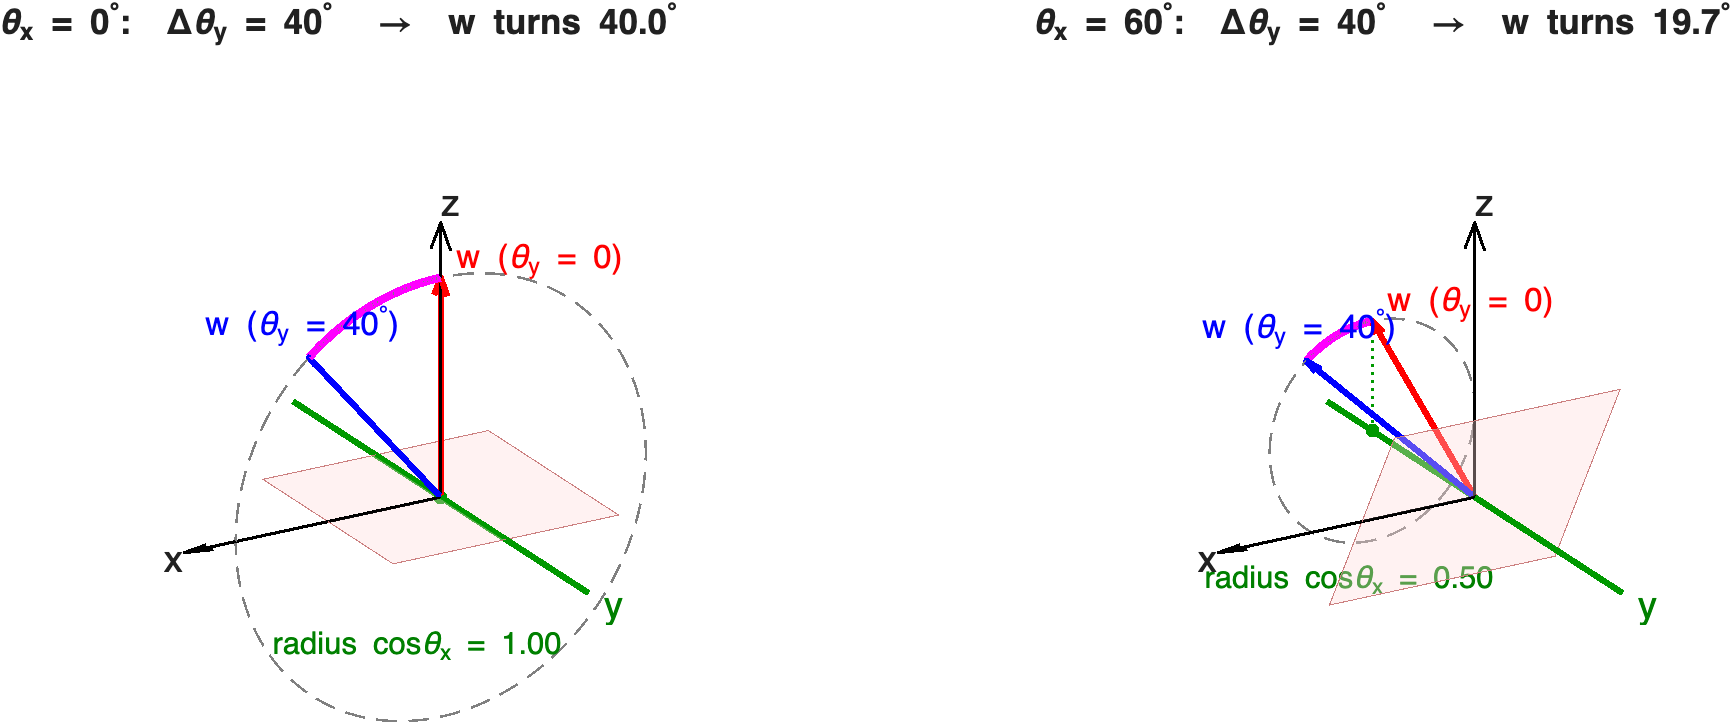
\includegraphics[width=0.9\textwidth]{fig_1023_cos_thetax_axes.png}
\end{center}

\section*{Comparison}
{\small
\begin{tabular}{@{}llll@{}}
\toprule
 & Notes (Word) & 1015 (angles as states) & This document \\
\midrule
States & ${}^{V}\delta\mathbf p$, $\boldsymbol\lambda$, $\boldsymbol\theta$ (local) & $\dpb$ (x, y, z), $\aT$, $\aN$, $\theta_x$, $\theta_y$ & $\dpb$, $\av$ (x, y, z) \\
Gain matrix & $\boldsymbol\lambda$ with $\V$ & $\Vh\,\mathrm{diag}(\haT, \haT, \haN)\,\Vh^{T}$ & six entries of $\Ah$ \\
Angles & states, measured $\theta_m$ & states, rows of ${}^{v}\Ab_m$ & computed from $\Ah$ (A5, closed form) \\
End of step & $\V[k]$ out, $\V^{T}[k+1]$ in & none & none \\
$\mathbf F_e$ & $\mathbf G_\lambda$, $\mathbf G_\theta$ & gain and angle columns, $\cos\hat\theta_x$ & force matrix only \\
$\mathbf H$ & selects ${}^{V}\delta\mathbf p_1$, $\boldsymbol\lambda$, $\boldsymbol\theta$ & angle rows $\haT - \haN$ & $\I_3$, $\I_6$ \\
\bottomrule
\end{tabular}
}

\end{document}
